\chapter{LAPS}
\section{Einleitung}
Local Administrator Password Solution (LAPS)

\subsection{Anforderungen}
Um LAPS einsetzten zu können, wir ein Active Directory benötigt.

\section{Installation}
Die Installation ist in drei Schritte unterteilt.
Als erstes wird LAPS per Group Policy auf allen Windows Geräten installiert.
Danach wird das Active Directory für LAPS vorbereitet und zum Schluss wird LAPS per Group Policy aktiviert.

\subsection{Softwareverteilung}

\begin{enumerate}
    \item LAPS kann auf der \href{https://www.microsoft.com/download/details.aspx?id=46899}{Webseite von Microsoft}\footnote{Link: https://www.microsoft.com/download/details.aspx?id=46899} heruntergeladen werden.
    \item Die Datei muss in einem freigegebenen Netzlaufwerk auf dem Domain Controller platziert werden, auf welches alle Computer zugriff haben.
          Zum Beispiel: C:\textbackslash Windows\textbackslash SYSVOL\textbackslash sysvol\textbackslash <domain>\textbackslash.
          Dieses Verzeichniss ist Standardmässig freigegeben.
    \item Im Group Policy Management muss eine neue Group Policy erstellt werden, welche mit der OU verknüpft ist, die alle Windows Geräte enthält.

    \item d
    \item d
    \item d
    \item d
\end{enumerate}
%TODO: Does not Work
%\begin{figure}[h]
%    \centering
%    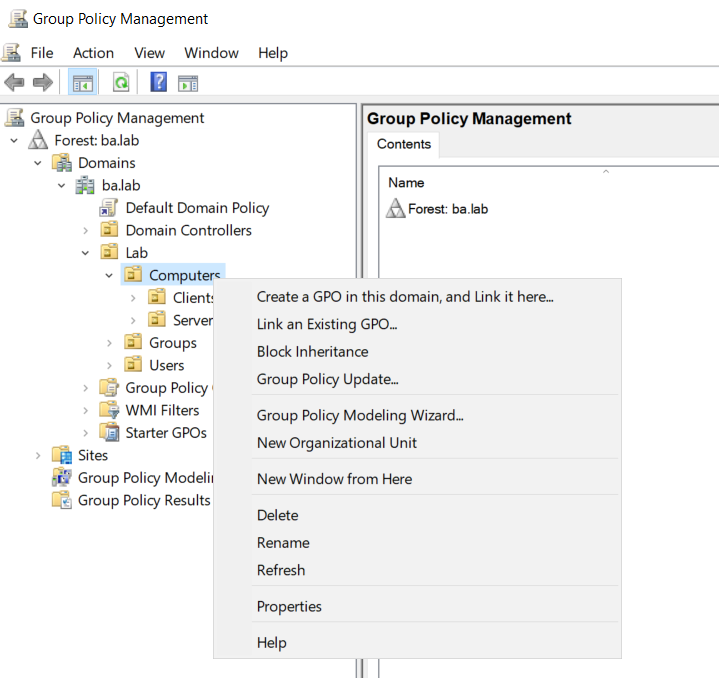
\includegraphics[width=0.7\linewidth]{LAPS/GPO-Create-New.png}
%    \caption{Neue GPO für LAPS Deployment}
%\end{figure}
%3. Open GPO Editor on DC and Create a new GPO+Link to all Computer OUs
%
%4. Edit GPO and add new Software Installation. Select .msi on path from before.
%
%5. Close GPO. PC will install after restart or force with gpupdate /force
%Hint: Install manually on DC to prevent restart.
%
%\subsection*{Install UI for Admins}
%
%1. Open Programm List
%2. Click LAPS and Change. Click Change [LAPS-UI-Install]
%3. Add Management Tools, Next, Change, Finish
%
%
%\section{Configure AD}
%
%1. Add Extension Attribute (Admin must be Schema Admin)
%
%2. Run commands
%Import-module AdmPwd.PS (If not available, LAPS not installed on DC)
%Update-AdmPwdADSchema
%
%Result:
%Operation            DistinguishedName                                                 Status
%---------            -----------------                                                 ------
%AddSchemaAttribute   cn=ms-Mcs-AdmPwdExpirationTime,CN=Schema,CN=Configuration,DC=b... Success
%AddSchemaAttribute   cn=ms-Mcs-AdmPwd,CN=Schema,CN=Configuration,DC=ba,DC=lab          Success
%ModifySchemaClass    cn=computer,CN=Schema,CN=Configuration,DC=ba,DC=lab               Success
%
%
%Set-AdmPwdComputerSelfPermission -OrgUnit "Clients"
%Name                 DistinguishedName                                                 Status
%----                 -----------------                                                 ------
%Clients              OU=Clients,OU=Computers,OU=Lab,DC=ba,DC=lab                       Delegated
%
%
%3. Create a Group where all Users are added, that can use LAPS. [Laps-Admins.png]
%
%4. Open ASedit [ASEdit.png] and Open Properties of OU with Computers. Open Security tab. Add Group and give ``All Extended Rights''
%Remove All Extended Rights on unneeded accounts
%
%5. Run:
%
%Set-AdmPwdReadPasswordPermission -OrgUnit "Clients" -AllowedPrincipals Global_LAPS-Admins
%Set-AdmPwdResetPasswordPermission -OrgUnit "Clients" -AllowedPrincipals Global_LAPS-Admins

%6. Check Permission:
%
%Find-AdmPwdExtendedrights -identity "Clients"
%
%
%\section{Enforce with GPO}
%
%1. Open GPO Editor on DC and Create a new GPO+Link to all Computer OUs
%
%2. Edit Policy and go to Computer Configuration > Policies > Administrative Templates > Laps [enable-laps]
%
%3. Enable Password Settings and define how: best 14 characters and change all
%
%
%